\section{Architektur des Microservice}
\label{sec: Architektur des Microservice}
Der Microservice Warenwirtschaft wurde in der Programmiersprache Go\footnote{https:\//golang.org\/doc\/} entwickelt. Go-An-wendungen bestehen aus Packages, in denen die einzelnen Go-Files organisiert sind, Klassen im Sinne der Objektorientierung gibt es nicht. Der Microservice Warenwirtschaft sett sich aus den neun Packages zusammen, die in der Abbildung X dargestellt werden. In den beiden nachfolgenden Unterkapiteln werden die Packages und die darin enthaltenen Go-Files des Presentation  sowie des Application Layers kurz vorgestellt. Go-Files mit der Bezeichnung \texttt{<<Name>>\_test.go} beinhalten Whitebox-Testfälle um die Funktionen der benannten Go-Files zu prüfen. Aus Gründen der Übersichtlichkeit werden diese File hier nicht explizit aufgeführt. 
Der Microservice nutzt anstelle einer klassischen Datenbank eine In-Memory-Datenbank im Cache. Aus diesem Grund verschwimmen klassischen Grenzen des Application und Persitant Layers und auf die dezidierte Aufführung des letzteren wird verzichtet.

\begin{figure}[H]
	\begin{center}
	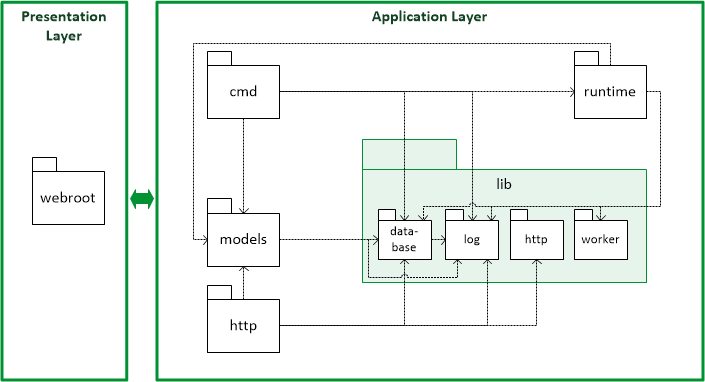
\includegraphics[width=0.65 \textwidth]{./pics/struktur.png}
	\end{center}
	\caption{Struktur des Microservice}
	\label{pic:Struktur des Microservice}
\end{figure}


\subsection{Schnittstellen zu anderen Microservices}
\label{subsec: Schnittstellen zu anderen Microservices}
Der Microservice Warenwirtschaft weißt vier Schnittstellen\footnote{Da es nicht Teil der übergeordneten Aufgabenstellung war, die Microservices der einzelnen Projektgruppen zu einem lauffähigen Webshop zusammenzufügen, greift der Microservice Warenwirtschaft an diesen Stellen auf Testdaten zurück} zu anderen Microservices auf. Zum einen sollte für die Authentifizierung der Benutzer des Admin-Frontends auf den Microservice Benutzerauthentifizierung zurückgegriffen werden. Außerdem benötigt der Microservice Informationen darüber, ob ein Benutzer eine Ware in den Warenkorb gelegt hat und ob eine Ware versandt wurde. Somit entstehen ebenfalls Schnittstellen zu den Microservices Bestellung und Versandt. Abschließend weißt dieser Microservice eine Schnittstelle zu dem Microservice Produktkatalog auf, von welchem die angebotenen Produkte -- die sich dementsprechend im Lager befinden können -- abgefragt werden.

\newpage
\subsection{Presentation Layer}
\label{subsec: Presentation Layer}
Der Presentation Layer umfasst alle  Packages, die sich mit der eigentlichen Darstellung der Warenwirtschaft aus der Sicht des Endbenutzers befassen. Im Detail ist dies das Package \textbf{\texttt{webroot}}, welches den statischen Inhalt der Frontends, wie zum Beispiel die HTML-Files und Bilder enthält.


\subsection{Application Layer}
\label{subsec: Application Layer}

\paragraph{cmd:} Go-File main.go, welches alle Angaben zu den Config-Files der Applikation enthält

\paragraph{http:} Go-Files, die die Anwendungslogik (Funktionen) und die API-Rounten beinhalten.
	\begin{itemize}
	\item \texttt{bindapi.go}: Funktionen, die für das Binden der URL-Pfade notwendig sind
	\item \texttt{good.go}: Funktionen fpr das Hinzufügen von Waren zum Warenbestand
	\item \texttt{good\_show.go}: Funktionen für die Auflistung und Zählung der vorhandenen Waren sowie die Feststellung ihrer Verfügbarkeit zusammen
	\item \texttt{good\_temp.go}: Hilfsfunktionen, die für die Darstellung des Warenbestandes als Ampel im Kunden-Frontend benötigt werden
	\item \texttt{status.go}: Funktion, die den Status des Microservice abfragt 
	\end{itemize}


\paragraph{models:} Go-Files, die Structs und zugehörige Hilfsfunktionen (hauptsächlich statischen Inhalt des Microservice) beinhalten 
	\begin{itemize}
	\item \texttt{config.go}: Structs mit den Informationen zur Konfiguration des Webservers, der Datenbank und dem Cache-Management sowie Hilfsfunktionen zum Lesen von Config-Files
	\item \texttt{duration.go}: Structs und Hilfsfunktionen zur Definition eines Typs für Zeitangaben
	\item \texttt{good.go}: Structs und Hilfsfunktionen zur Darstellung von Waren, hier werden auch die beschriebenen Funktionalitäten wie das Blockieren von Waren beschrieben
	\item \texttt{structstorage}: 
	\end{itemize}


\paragraph{runtime:} Go-Files mit weiteren Hilfsfunktionen
	\begin{itemize}	
	\item \texttt{auth.go}: Hilfsfunktionen zur Prüfung, ob eine Berechtigung für den Zugriff vorliegt
	\item \texttt{cache\_worker.go}: Hilfsfunktionen für das Löschen und Anlegen von Cache-Workers
	\item \texttt{good\_release.go}: Hilfsfunktionen zum Blockieren und Entsperren Waren
	\item \texttt{productcache.go}: Hilfsfunktionen zum Anlegen eines Caches für Produkte und zur Prüfung
	\item \texttt{runtime.go}: Übergreifende Hintergrundfunktionalitäten	
	\end{itemize}
	


\newpage
\paragraph{lib:} fasst die vier Packages \texttt{database}, \texttt{http}, \texttt{log} und \texttt{worker} zusammen

	\begin{itemize}
	\item \texttt{database}: Go-File \texttt{database.go} mit Funktionen für das Öffnen und Schließen der Datenbank
	\item \texttt{http}: Go-Files, die die Webserverlogik umgesetzten
		\begin{itemize}
		\item \texttt{io.go}: Funktionen zum Lesen und Schreiben von JSON aus beziehungsweise in HTTP-PAckete
		\item \texttt{permission.go}: Funktionen zur Prüfung der Berechtigung für den Zugriff
		\end{itemize}	
	\item \texttt{log}: Go-File \texttt{log.go}, das den Logger startet und initiiert
	\item \texttt{worker}: Go-File \texttt{worker.go}, dass Funktionen für die Nutzung des Caches für die Produkte aus dem Produktkatalog (Worker) bereitstellt 
	\end{itemize}

\subsection{Integrierte Tests}
\label{subsec: Integrierte Test}
Neben den Go-Files die bereits Whitebox-Tests enthalten, ist in dem Package \textbf{\texttt{test}} ein weiteres Go-File (\texttt{testrest.go}) enthalten. Dieses setzt einen Test des Webservers um, bei dem auf Testdaten eines Produktkataloges zurückgegriffen wird. Mit Hilfe der integrierten Test kann in der hier beschriebenen Version eine Code-Coverage von 100\% erreicht werden, das heißt jedes Stück Code wird mindestens einmal zur Ausführung gebracht.

\subsection{Admin-Frontend}
\label{subsec: Admin-Frontend}



\subsection{Anpassung des Monolithen}
\label{subsec: Anpassung des Monolithen}
